\documentclass[11pt,preprint, authoryear]{elsarticle}

\usepackage{lmodern}
%%%% My spacing
\usepackage{setspace}
\setstretch{1.2}
\DeclareMathSizes{12}{14}{10}{10}

% Wrap around which gives all figures included the [H] command, or places it "here". This can be tedious to code in Rmarkdown.
\usepackage{float}
\let\origfigure\figure
\let\endorigfigure\endfigure
\renewenvironment{figure}[1][2] {
    \expandafter\origfigure\expandafter[H]
} {
    \endorigfigure
}

\let\origtable\table
\let\endorigtable\endtable
\renewenvironment{table}[1][2] {
    \expandafter\origtable\expandafter[H]
} {
    \endorigtable
}


\usepackage{ifxetex,ifluatex}
\usepackage{fixltx2e} % provides \textsubscript
\ifnum 0\ifxetex 1\fi\ifluatex 1\fi=0 % if pdftex
  \usepackage[T1]{fontenc}
  \usepackage[utf8]{inputenc}
\else % if luatex or xelatex
  \ifxetex
    \usepackage{mathspec}
    \usepackage{xltxtra,xunicode}
  \else
    \usepackage{fontspec}
  \fi
  \defaultfontfeatures{Mapping=tex-text,Scale=MatchLowercase}
  \newcommand{\euro}{€}
\fi

\usepackage{amssymb, amsmath, amsthm, amsfonts}

\def\bibsection{\section*{References}} %%% Make "References" appear before bibliography


\usepackage[round]{natbib}

\usepackage{longtable}
\usepackage[margin=2.3cm,bottom=2cm,top=2.5cm, includefoot]{geometry}
\usepackage{fancyhdr}
\usepackage[bottom, hang, flushmargin]{footmisc}
\usepackage{graphicx}
\numberwithin{equation}{section}
\numberwithin{figure}{section}
\numberwithin{table}{section}
\setlength{\parindent}{0cm}
\setlength{\parskip}{1.3ex plus 0.5ex minus 0.3ex}
\usepackage{textcomp}
\renewcommand{\headrulewidth}{0.2pt}
\renewcommand{\footrulewidth}{0.3pt}

\usepackage{array}
\newcolumntype{x}[1]{>{\centering\arraybackslash\hspace{0pt}}p{#1}}

%%%%  Remove the "preprint submitted to" part. Don't worry about this either, it just looks better without it:
\makeatletter
\def\ps@pprintTitle{%
  \let\@oddhead\@empty
  \let\@evenhead\@empty
  \let\@oddfoot\@empty
  \let\@evenfoot\@oddfoot
}
\makeatother

 \def\tightlist{} % This allows for subbullets!

\usepackage{hyperref}
\hypersetup{breaklinks=true,
            bookmarks=true,
            colorlinks=true,
            citecolor=blue,
            urlcolor=blue,
            linkcolor=blue,
            pdfborder={0 0 0}}


% The following packages allow huxtable to work:
\usepackage{siunitx}
\usepackage{multirow}
\usepackage{hhline}
\usepackage{calc}
\usepackage{tabularx}
\usepackage{booktabs}
\usepackage{caption}


\newenvironment{columns}[1][]{}{}

\newenvironment{column}[1]{\begin{minipage}{#1}\ignorespaces}{%
\end{minipage}
\ifhmode\unskip\fi
\aftergroup\useignorespacesandallpars}

\def\useignorespacesandallpars#1\ignorespaces\fi{%
#1\fi\ignorespacesandallpars}

\makeatletter
\def\ignorespacesandallpars{%
  \@ifnextchar\par
    {\expandafter\ignorespacesandallpars\@gobble}%
    {}%
}
\makeatother

\newlength{\cslhangindent}
\setlength{\cslhangindent}{1.5em}
\newenvironment{CSLReferences}%
  {\setlength{\parindent}{0pt}%
  \everypar{\setlength{\hangindent}{\cslhangindent}}\ignorespaces}%
  {\par}


\urlstyle{same}  % don't use monospace font for urls
\setlength{\parindent}{0pt}
\setlength{\parskip}{6pt plus 2pt minus 1pt}
\setlength{\emergencystretch}{3em}  % prevent overfull lines
\setcounter{secnumdepth}{5}

%%% Use protect on footnotes to avoid problems with footnotes in titles
\let\rmarkdownfootnote\footnote%
\def\footnote{\protect\rmarkdownfootnote}
\IfFileExists{upquote.sty}{\usepackage{upquote}}{}

%%% Include extra packages specified by user

%%% Hard setting column skips for reports - this ensures greater consistency and control over the length settings in the document.
%% page layout
%% paragraphs
\setlength{\baselineskip}{12pt plus 0pt minus 0pt}
\setlength{\parskip}{12pt plus 0pt minus 0pt}
\setlength{\parindent}{0pt plus 0pt minus 0pt}
%% floats
\setlength{\floatsep}{12pt plus 0 pt minus 0pt}
\setlength{\textfloatsep}{20pt plus 0pt minus 0pt}
\setlength{\intextsep}{14pt plus 0pt minus 0pt}
\setlength{\dbltextfloatsep}{20pt plus 0pt minus 0pt}
\setlength{\dblfloatsep}{14pt plus 0pt minus 0pt}
%% maths
\setlength{\abovedisplayskip}{12pt plus 0pt minus 0pt}
\setlength{\belowdisplayskip}{12pt plus 0pt minus 0pt}
%% lists
\setlength{\topsep}{10pt plus 0pt minus 0pt}
\setlength{\partopsep}{3pt plus 0pt minus 0pt}
\setlength{\itemsep}{5pt plus 0pt minus 0pt}
\setlength{\labelsep}{8mm plus 0mm minus 0mm}
\setlength{\parsep}{\the\parskip}
\setlength{\listparindent}{\the\parindent}
%% verbatim
\setlength{\fboxsep}{5pt plus 0pt minus 0pt}



\begin{document}



\begin{frontmatter}  %

\title{Time-varying Correlation of South African Property Stocks (REITs)
and the JSE FTSE All Share Index (ALSI)}

% Set to FALSE if wanting to remove title (for submission)




\author[Add1]{Andrew Hyde}
\ead{23365935@sun.ac.za}





\address[Add1]{Stellenbosch University, South Africa}


\begin{abstract}
\small{
The study investigates the strong performance of South African property
returns stocks after the REITs legislation came into affect in 2013 as
well as the subsequent loss of value of property stocks experience from
2018. Additionally this paper makes use of a DCC GARCH model to explore
the relationship between REITs and the rest of the ALSI equities on the
Johannesburg Stock Exchange (JSE) to explain the role that REITs or
property stocks can serve on a mixed asset portfolio using returns data
from the JSE FTSE All Share Index.
}
\end{abstract}

\vspace{1cm}





\vspace{0.5cm}

\end{frontmatter}



%________________________
% Header and Footers
%%%%%%%%%%%%%%%%%%%%%%%%%%%%%%%%%
\pagestyle{fancy}
\chead{}
\rhead{}
\lfoot{}
\rfoot{\footnotesize Page \thepage}
\lhead{}
%\rfoot{\footnotesize Page \thepage } % "e.g. Page 2"
\cfoot{}

%\setlength\headheight{30pt}
%%%%%%%%%%%%%%%%%%%%%%%%%%%%%%%%%
%________________________

\headsep 35pt % So that header does not go over title




\hypertarget{introduction}{%
\section{\texorpdfstring{Introduction
\label{Introduction}}{Introduction }}\label{introduction}}

Real Estate Investment Trusts (REITs) around the world have become a
popular investment vehicle to gain exposure to public real estate as an
asset class. REITs were first created in the United States in 1960 as an
investment vehicle to provide both institutional and retail investors
with an accessible means of investing in income-producing real estate
(Carstens and Wesson, 2019). What followed was the introduction of REITs
in other countries such as Australia, Canada, Germany, Singapore etc.
(National Treasury, 2007). Included in this list was South Africa, which
introduced this type of listed property investment security in May 2013.

In South Africa, before the introduction of REITs, the most established
types of property investment securities listed on the Johannesburg Stock
Exchange (JSE) were Property Loan Stocks (PLSs) and Property Unit Trusts
(PUTs) (National Treasury, 2007). Both these two types of common
property investment vehicles suffered from tax inconsistencies, as PLSs
paid capital gains tax on property sales and PUTs did not have this tax
incidence (National Treasury, 2007). Overall, the property investment
landscape was seen to be restrictive and lacked the regulatory structure
to compete for capital on an international scale (Bredell and Boshoff,
2013). The introduction REITs offered investors, both foreign and
domestic, greater opportunities to invest in the South African property
market.

The reason for the introduction of REITs was the benefits associated
with this securities design. REITs offered an accessible, safe, and
simple means by which investors could invest in the property market
(National Treasury, 2007). The structure of this listed security
enhanced its liquidity as it can be traded daily on the JSE and offered
predictable income streams, while offering opportunities for
diversification (Bredell and Boshoff, 2013). This combined with the tax
efficiencies over PUTs and PLSs, saw the number of listed property
stocks rise in popularity in South Africa to the extent where today they
make included in broader indexes such as the JSE All Share Index (ALSI),
JSE Shareholder Weighted Index (SWIX) and JSE FTSE Top 40 Index
(Carstens and Wesson, 2019).

The inclusion of REITs in such indexes alongside other traditional
listed equities, that share similar regulations, has been questioned
given that REITs are subjected to significantly different regulations.
SA REITs are required to generate at least 75\% of total income from
immovable property and 75\% of assets held by REITs must be immovable
property such as shopping centres, office buildings and residential
developments (Bredell and Boshoff, 2013). Additionally, REITs are
required to invest in immovable property for the long term as opposed to
speculative trading of properties (National Treasury, 2007). Concerning
distributions of earnings, REITs are obligated to distribute more than
75\% of earnings as dividends. In terms of debt, REITs are subjected to
a gearing limit of 60\% of debt to gross asset value (National Treasury,
2007).

The structure of the regulations governing REITs made this investment
vehicle attractive. The adoption of these regulations had the
implication of creating listed securities that offer higher dividends
than predecessors property investment vehicles, experience lower
volatility due to steady income streams, are seen as a cost-effective
means of gaining exposure to property in one's portfolio, and lower
entry and exit costs (Bredell and Boshoff, 2013). Additionally, REITs
offer a diversified alternative to directly holding property due to
multiple property holdings with a diversified tenant pool and by
implication diversified income stream. According to Katzler and Song
(2019), public real estate exhibit favorable risk-return characteristics
and lower correlations with other financial assets such as equities and
fixed income. The qualities that property poses as an asset class can
aid in portfolio diversification through matching assets with low
correlation profiles or even negative correlation profiles, and
therefore provides an advantage of including public real estate in a
mixed asset portfolio (Katzler and Song, 2019). The benefit of
diversifying one's portfolio with REITs would then be based on its lower
correlation with other assests. While these characteristics do provide
an incentive to investors to include REITs as part of a mixed asset
portfolio, a question that arises is whether REITs do indeed offer
exposure to public property or are more similar to traditional listed
equities in terms of their return profiles (Deng, Ding and Fei, 2010).

The purpose of this paper is twofold. First, to provide an explanation
for the strong performance of property returns stocks after the REITs
legislation came into effect in 2013 and fro the subsequent loss of
value of property stocks experience from 2018. Second, to explore the
relationship between REITs and the rest of the ALSI equities on the
Johannesburg Stock Exchange (JSE) to explain the role that REITs or
property stocks serve on a mixed asset portfolio. More specifically to
determine how the conditional correlation between the equity pairs
changes over time. The model used to conduct this analysis is a Dynamic
Conditional Correlation Generalized AutoRegressive Conditional
Heteroskedasticity (DCC GARCH) model on returns data from the JSE FTSE
All Share Index to generate time-varying conditional correlation
estimates.

The paper is structure as follows: Section 2 provides a literature
review and brief analysis of the performance history of REITs. Section 3
describes the data and methodology used in the study. Section 4 provides
discusses and presents the results of the analysis. Finally, Section 5
concludes the findings of the paper.

\hypertarget{historical-performance-of-south-african-property-stocks}{%
\section{Historical Performance of South African Property
Stocks}\label{historical-performance-of-south-african-property-stocks}}

In 2013, once the REIT regulation took affect the popularity and
performance of SA REITs was the public property sectors inclusion in
mixed asset portfolios increase substantially. As seen in Figure 3.1,
the cumulative returns of REIT equities performed well and in fact
outperformed the rest of the JSE FTSE All Share Index (ALSI) excluding
REITs. Given the indexes weights are construction using market
capitalization, it is important to bear in mind that the ALSI is heavily
weighted in favour of listed companies with large market capitalization
of their shares. With sectors such as resources being weighted heavily,
due to their market capitalization, then results can be explained by the
performance of the resources sector or the commodity cycle. Figure 2.2
provides credence to this insights as the plotted resources cumulative
returns closely resembles that of the ALSI seen in Figure 2.1.

From 2013, management of REITs faced a globally competitive environment
with high-growth pressure coming from the expected returns of investors
(Carstens and Wesson, 2019). Management of REITs responded in two ways
to this pressures and these responses can be relate to the REIT
legislation. The results was that from 2014 and 2015 SA REITs market
capitalization increased by 47\% (Carstens and Wesson, 2019).

Firstly, in terms of distributions REITs earnings, pay-out ratios from
2013 to 2018 were at 100\% despite the minimum requirement of 75\%.
According to Head of STANLIB Listed Property, Keillen Ndlovu (2019),
since the introduction of REITs typically 100\% of earnings were
distributed to investors whereas in other countries typically only paid
out between 75\% and 90\%. This ended in 2018 when Delta Property Fund
decaresed their pay-out to the minimum of 75\% (Ndlovu 2019). Thus, SA
REITs have not made use of earnings to fund portions of their operations
or services debt in an attempt to bolster share prices and have instead
finance expansion through debt.

Secondly, the average debt to gross asset ratio of the vast majority of
REITs increased from a low of 27\% to 40\% by July 2019 (Ndlovu, 2019),
bearing in mind that the limit is 60\%. Given the market's search for
returns, SA REITS expanded their gross asset holding considerably
through acquisitions and new developments particularly in the commercial
and retail property spaces (Carstens and Wesson, 2019). This resulted in
increased share price returns for investors as high future income growth
was priced in as the rapid expansion progressed. What soon became the
case was that the South African market became over supplied with
commercial and retail properties and REITs undertook purchases of
foreign property assets to diversify their own income streams and by
2019, global exposure of the SA REIT market was 47\% from being
virtually zero a decade prior (Ndlovu, 2019).

By 2018, the SA REIT market was heavily indebted and unable to lease out
the oversupplied commercial and retail space. Investors had started
pricing in declining growth of future rental income streams and at the
time interest had increased with the repo rate increasing from 5\% in
2013 to a year high of 6.75\% in 2018 (SARB, 2023). In early 2018,
concerns mounted for the high debt ratios of REITs given decreases
experienced in rental income that lead fund managers to quickly exit
positions of REIT holdings driving share prices downwards by doing so
(Ndlovu, 2019). What followed was that REITs began to pay of debt and
thereby de-leveraging their operations which resulted in decreased
dividend payouts with the result being further decreases in the stock
prices of REITs and the sector losing over 25\% of its value by the end
of 2018 (Ndlovu, 2019). In 2020, REITs experienced a further blow as the
COVID-19 pandemic reduced the demand of office space as hybrid work
models were established and the pace at which retailers expanded there
online stores increased rapidly, and subsequently the demand for retail
space fell as well. Figure 2.3 highlights these developments in the
REITs sector through plotting the noise reduced volatility of property
stocks over time.

\begin{figure}
\centering
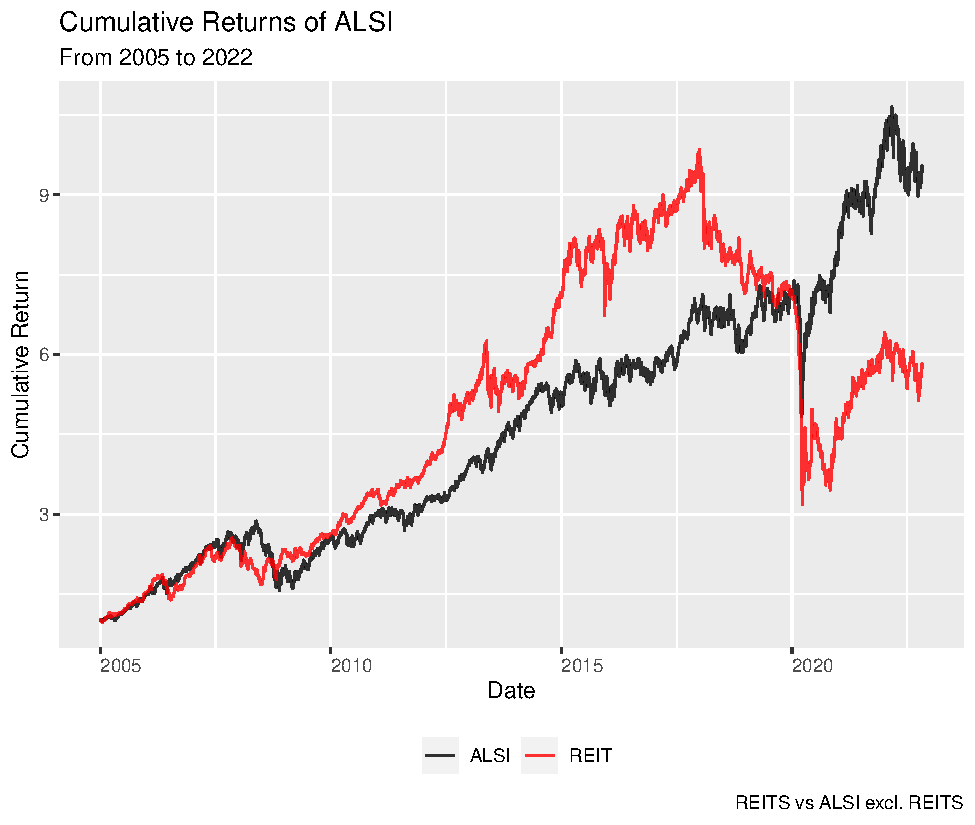
\includegraphics{Fin_Metrics_Project_files/figure-latex/unnamed-chunk-1-1.pdf}
\caption{Cumulative Returns}
\end{figure}

\hypertarget{initial-analysis-of-the-reits-sector}{%
\subsection{Initial Analysis of the REITs
Sector}\label{initial-analysis-of-the-reits-sector}}

The South African ALSI is heavily weighted by resources and the
performance of resource stocks can be explained by the time line of the
the commodity price cycle as these stock prices are heavily influenced
by the prices of the commodities they produce and sell. Prior to the
Global Financial Crisis (GFC) in 2008 the demand for commodities was
high during this period often referred to as the end of the great
moderation as economies around the world experiencing substantial
increases in economic growth and infrastructure developments. After
2008, global demand for commodities did not experience the same growth
as they did prior to the GFC. After the COVID pandemic the demand for
resources increased substantially and the performance of resources
stocks improve in kind.

From Figure 2.2, the cumulative returns of resources and property stocks
appear to move in opposite directions. A possible explanation maybe be
related to property building costs and the logic would be as follows.
When commodity or resources prices are cheap the cost to construct
property is lower and therefore REITs would perform well with some lag.
However, upon further investigation this does not seem plausible as the
dynamic condition correlation between the property and resources, which
is displayed in Figure 4.2, is significantly low but this cannot be
entirely dismissed unless the correlation structure is explored between
returns of resources and lagged property stock returns.

\begin{figure}
\centering
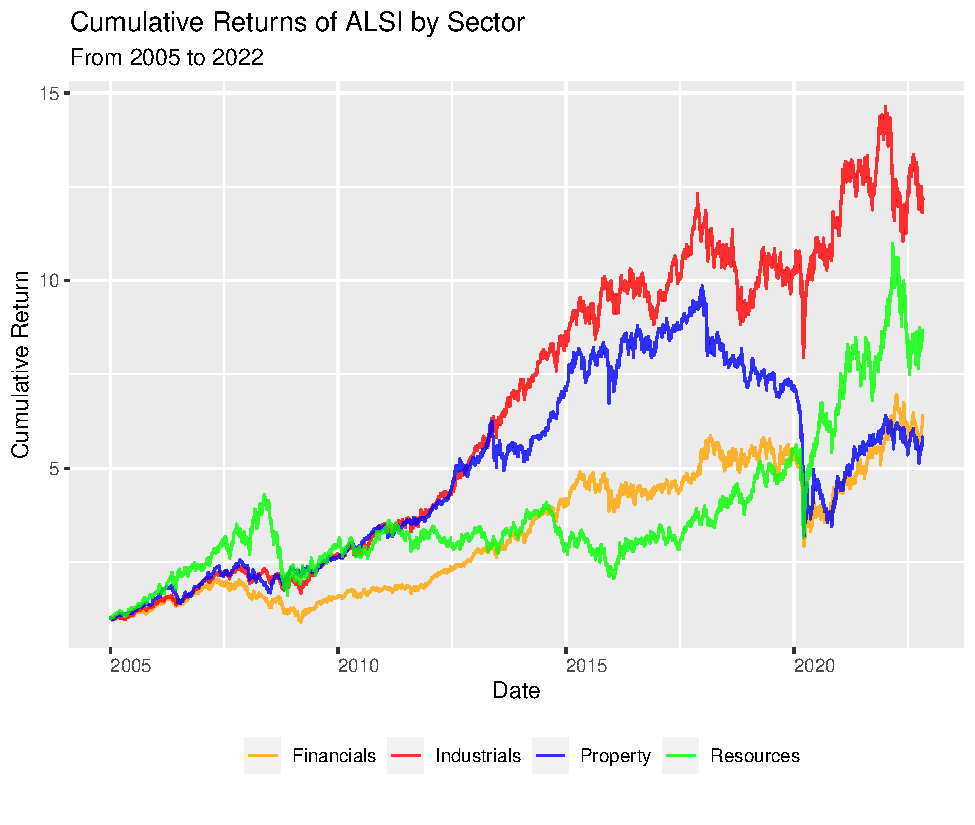
\includegraphics{Fin_Metrics_Project_files/figure-latex/unnamed-chunk-2-1.pdf}
\caption{Cumulative Returns}
\end{figure}

When comparing noise reduce volatility in Figure 2.3, the All Share
Index in South Africa experiences lower levels of volatility from 2005
to 2013. After 2013, SA REITs returns begin to experience highly
volatile periods until the end of the sample period. From Figure 2.3,
since 2013 there have have been four distinct spikes in volatility. The
first being around the time the REIT regulation taking affect in May
2013 (Treasury, 2007). The second coinciding with the introduction of
three REITs into the JSE FTSE Top 40 Index, taking the total number of
REITs included in the index to five (Carstens and Wesson, 2019). The
third, occurring in 2018 when REIT share prices lost considerable value
(Ndlovu, 2019). Finally, the fourth inline with the COVID pandemic
timeline and the lock down that took place.

\begin{figure}
\centering
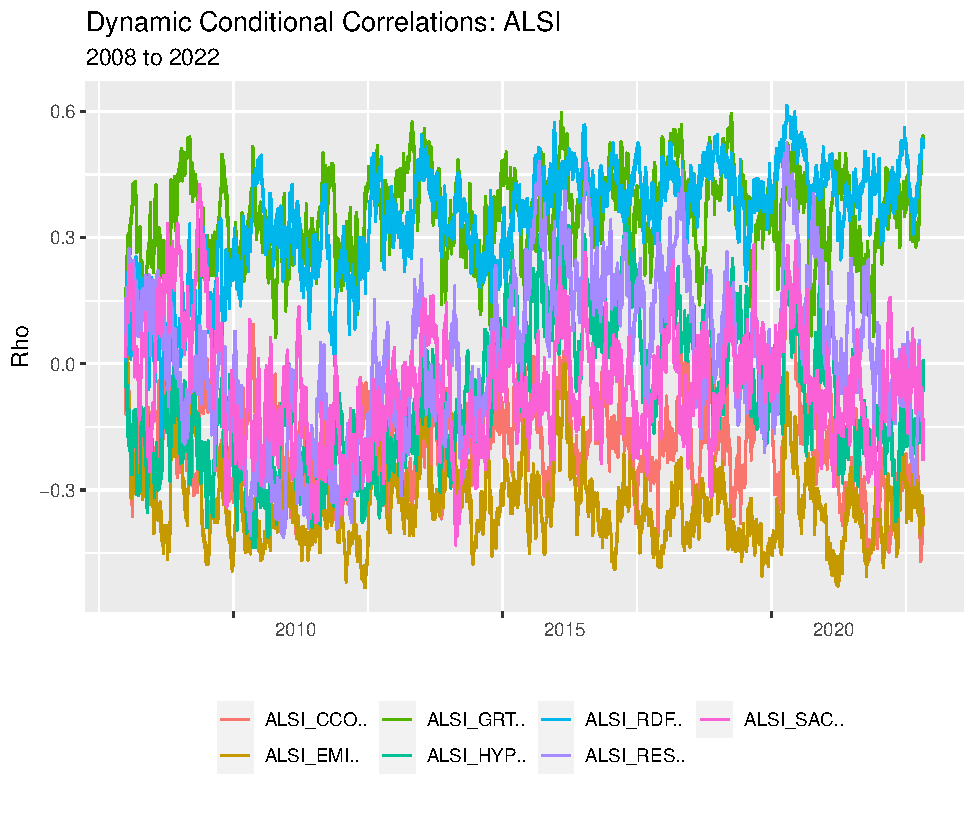
\includegraphics{Fin_Metrics_Project_files/figure-latex/unnamed-chunk-4-1.pdf}
\caption{Noise Reduced Volatility}
\end{figure}

\hypertarget{data-and-methodology}{%
\section{\texorpdfstring{Data and Methodology
\label{Methodology}}{Data and Methodology }}\label{data-and-methodology}}

\hypertarget{data}{%
\subsection{Data}\label{data}}

The dataset used in this study is the JSE FTSE ALSI returns data from
2005 to 2022, which included both traditional equities and REITs. An
investigation into the data reveals that there are four unique sectors
in the data, namely; Financials, Industrials, Resources and Property.
The JSE FTSE ALSI is the primary share index of the South Africa market.
The share index represents approximately the 99\% of the largest
companies subject to subject to minimum liquity and free float
standards, where each listed company is weighted by its own market
capitalisation against the summation of the market capitalisations of
all companies within the index (FTSE Russel, 2023).

The Figure in Annexure A, displays the available data for each REIT. In
the second half of the analysis Based on availability of data the
following REITs are selected: Capital \& Counties Properties PLC, Hyprop
Investments Limited, Growthpoint Properties Limited, Resilient Reit
Limited, Redefine Properties Limited, SA Corporate Real Estate Limited
and Vukile Property Fund Limited.

\hypertarget{methodology}{%
\subsection{Methodology}\label{methodology}}

A Dynamic Conditional Correlation Generalized AutoRegressive Conditional
Heteroskedasticity (DCC GARCH) model is used to perform this analysis.
This model allows for the estimation of time-varying conditional
correlation structures that are noise reduced, taking the GARCH(1,1)
model further by allowing for multivariate volatility modeling (Engle,
2002; Katzke, 2022c).

The DCC model makes use of non-Linear combinations of univariate GARCH
models to directly model the correlations as a dynamic time-varying
process i.e.~estimating the conditional correlation matrix directly
(Engle, 2002)

The DCC GARCH model follows a two-step approach.

\hypertarget{step-one}{%
\subsubsection{Step One}\label{step-one}}

Estimates are obtained by fitting a univariate GARCH(1,1) model to the
residuals of the vector autoregression (VAR) using the combined imputed
data. The VAR allows for the examination of relationships between series
over time and the residuals it produces \(\alpha_{t}\) can be broken
down into the structural volatility component \(z_{t}\) and the noise
component \(\mu_{t}\), provided \(\alpha_{t}\) are white noise
errors/residuals Katzke, 2022b).

The DCC GARCH model is defined as follows:

\[
H_{t}=D_{t}. R_{t}. D_{t},
\]

where \(H_{t}\) is positive definite variance-covariance matrix which is
splits into identical diagonal matrices \(D_{t}\) and \(R_{t}\), the
time-varying correlation estimates. The estimation of \(R_{T}\) requires
it to be inverted at each estimated period, therefore a proxy similar to
a GARCH(1,1), denoted by \(Q_{i j, t}\), is to be used (Engle, 2002).

\[
\begin{aligned}
Q_{i j, t} & =\bar{Q}+a\left(z_{t-1} z_{t-1}^{\prime}-\bar{Q}\right)+b\left(Q_{i j, t-1}-\bar{Q}\right) \\
& =(1-a-b) \bar{Q}+a z_{t-1} z_{t-1}^{\prime}+b . Q_{i j, t-1}
\end{aligned}
\]

Where \(Q_{i j, t}\) the unconditional (sample) variance estimate
between series \(i\) and \(j\), and \(\bar{Q}\) is the unconditional
matrix of standardized residuals from each univariate pair estimate.

The following equation is used to estimate \(R_{t}\):

\[
R_{t}=\operatorname{diag}\left(Q_{t}\right)^{-1 / 2} Q_{t} . \operatorname{diag}\left(Q_{t}\right)^{-1 / 2} .
\]

Which has bivariate elements:

\[
R_{t}=\rho_{i j, t}=\frac{q_{i, j, t}}{\sqrt{q_{i i, t} \cdot q_{j j, t}}}
\]

The resulting DCC model is then formulated as:

\[
\begin{aligned}
\varepsilon_{t} & \sim N\left(0, D_{t} \cdot R_{t} \cdot D_{t}\right) \\
D_{t}^{2} & \sim \text { Univariate GARCH }(1,1) \text { processes } \forall(\mathrm{i}, \mathrm{j}), \mathrm{i} \neq \mathrm{j} \\
z_{t} & =D_{t}^{-1} \cdot \varepsilon_{t} \\
Q_{t} & =\bar{Q}(1-a-b)+a\left(z_{t}^{\prime} z_{t}\right)+b\left(Q_{t-1}\right) \\
R_{t} & =\operatorname{Diag}\left(Q_{t}^{-1}\right) \cdot Q_{t} . \operatorname{Diag}\left(Q_{t}{ }^{-1}\right)
\end{aligned}
\]

\hypertarget{step-two}{%
\subsubsection{Step Two}\label{step-two}}

Using the standardized residuals from step one, the dynamic,
time-varying conditional correlations estimates can be obtained using a
log-likelihood approach.

The volatility approximation series that is estimated \(H_{t}\), can
then be standardized and used in fitting a DCC model for \(\eta_{t}\)
(Katzke, 2022c).

\[
\eta_{i, t}=\frac{\hat{\alpha_{i, t}}}{\hat{\sigma_{i, t}}}
\]

The DDC GARCH model is run twice. The first iteration models the
time-varying conditional correlation structure between the ALSI and
REITs, as well as the time-varying correlation structure between the
seven individual REITs included in the study.The second applies a
stratification method to the data before the DCC GARCH model is re-run.
The stratification methods enables one to examine how these time-varying
conditional correlation structure change in periods of low and high
volatility.

The stratification technique is used to isolate return dates when South
African markets experienced high levels of volatility. To do this, the
South African Rand is used as a benchmark index and is filtered for its
own top and bottom quantile (20\%) by monthly standard deviation of Rand
volatility. These dates are then used to filter the ALSI\_returns into
dates with low and high volatility. The code used in this section
follows a practical covered in Financial Econometrics 871 (Katzke,
2022a).

Following the stratification, the time-varying conditional correlation
structure is mapped between Capital \& Counties Properties PLC
(Capco/CCO) and both the ALSI and other SA listed REITs. This section
further explores the relationship between Capital \& Counties Properties
PLC, a UK based REIT and Redefine Properties Limited, an SA based REIT,
whom are both listed on the JSE.

\hypertarget{results-and-discussion}{%
\section{\texorpdfstring{Results and Discussion
\label{Results}}{Results and Discussion }}\label{results-and-discussion}}

The following sections explores the results of the DCC GARCH model for
different iterations of input data to explore the time-varying
correlations of REITs. This section follows a top-down approach
exploring the time-varying relationship between REITs and the ALSI as a
whole, correlation between individual JSE listed REITS, periods of low
and high volatility and between individual JSE listed REITs with the
bulk of there operations in different geographic areas such as
countries.

\hypertarget{time-varying-correlation-reits-and-alsi}{%
\subsection{Time-varying Correlation: REITs and
ALSI}\label{time-varying-correlation-reits-and-alsi}}

From the results of the DCC GARCH model plotted in Figure 4.1, the
current average correlation of the REITs sector with the JSE FTSE ALSI
excluding REITs is approximately between 50\% and 60\%. This
significantly higher from the approximate average correlation
coefficient of 0.3 in 2013. What this may reveals is that through there
expansion into new developments, acquisition of assets, increased liquid
and marker capitalization as well as offshore holdings REITs have come
to be more influence by similar macroeconomic variables to other listed
equities. What can also be noted from Figure 2.3, is that REITs returns
do appear experience more volatility then the ALSI excluding REITs.

\begin{figure}
\centering
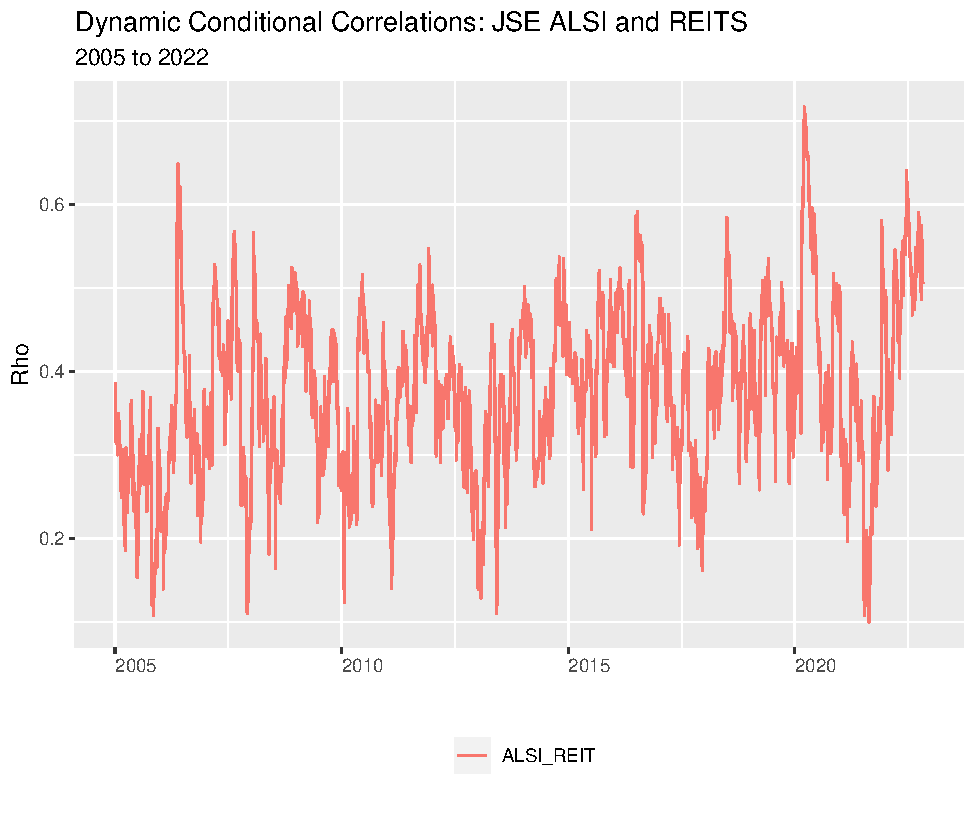
\includegraphics{Fin_Metrics_Project_files/figure-latex/unnamed-chunk-6-1.pdf}
\caption{Dynamic Conditional Correlations Graph}
\end{figure}

A significantly strong relationship exists between the returns of
financials and property stocks and has gained strength overtime. This is
evident by the results displayed in Figure 4.2, the current approximate
average correlation coefficient of 0.6 between the sector pair is
stronger than between property returns and resources or industrial. This
may be due to the similarities in the way that property and financials
operate as both are both asset heavy businesses that make use of
considerable amounts of leverage to scale their activities, they both
charge semi-fixed rates whether it be interest or rentals that can be
subject to escalations due to repo rate increases and finally, both
experience economic down due to similar macroeconomic variables in the
form of debtor defaults or property vacancies. This should not comes as
a surprise as sell-side equity specialists that focus on financials
typically cover property as well given there similarity in terms of
business models and income structures. Therefore, for the sake of
improving diversification one should be mindful what property and
financials stocks are held due to this increasing correlation trend and
one may consider holding more resources with property if prove to be
less correlated when controlled for with a lag.

\begin{figure}
\centering
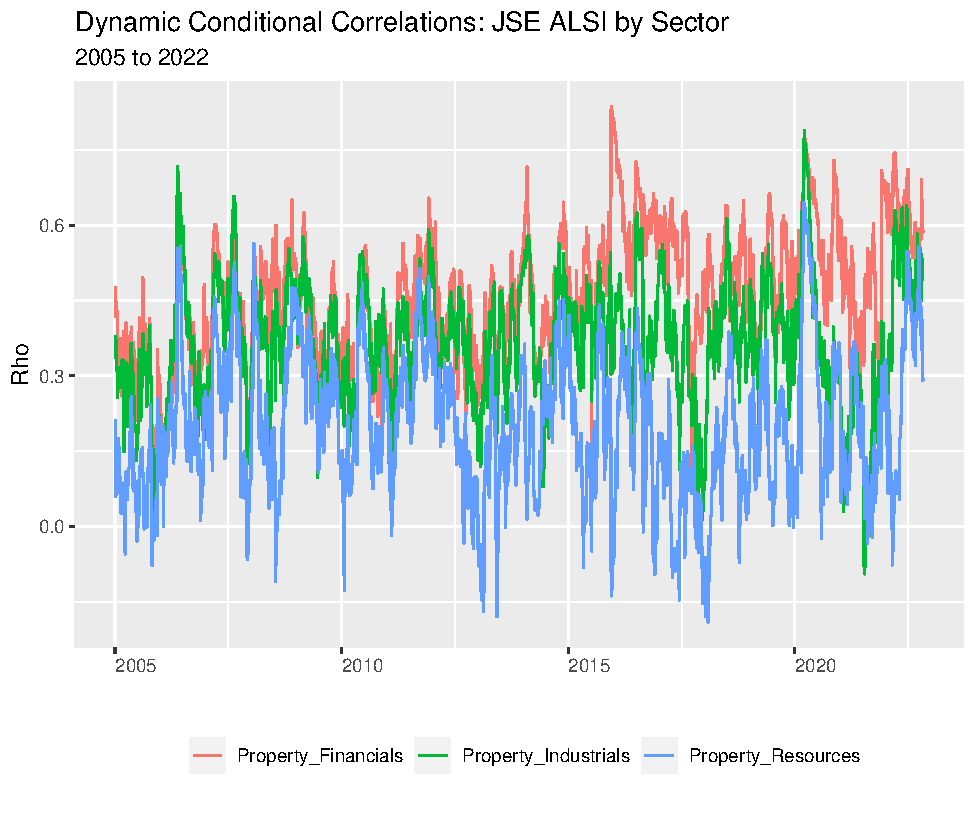
\includegraphics{Fin_Metrics_Project_files/figure-latex/unnamed-chunk-8-1.pdf}
\caption{Dynamic Conditional Correlations Graph}
\end{figure}

\hypertarget{individual-propert-stocks}{%
\subsection{Individual Propert Stocks}\label{individual-propert-stocks}}

The REITs used to plot Figure 4.3 are selected for their long standing
in the South African property market. Since the REIT regulation took
effect in 2013, have all experience consistent correlation coefficient
until the end of 2022. However, it is difficult to provide any analysis
about these individual property stocks from this figure. Therefore the
analysis turns to the individaul plotting of the time-varying
conditional correlation coefficeints of each stocks with the ALSI
excluding REITs.

\begin{figure}
\centering
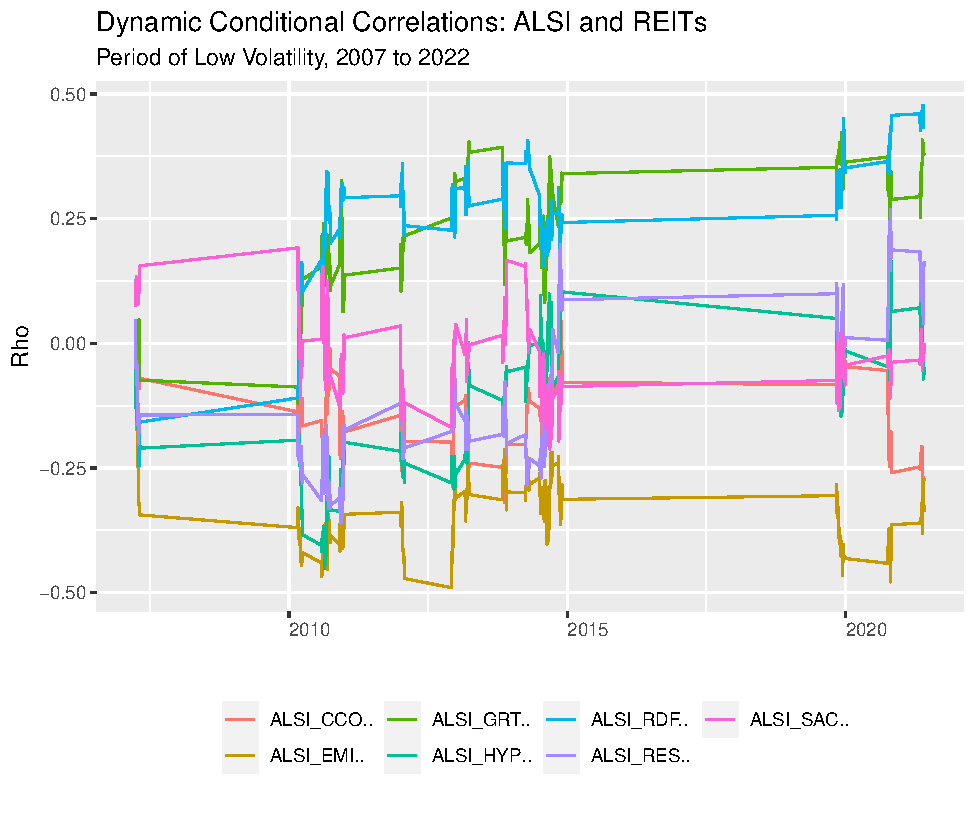
\includegraphics{Fin_Metrics_Project_files/figure-latex/unnamed-chunk-10-1.pdf}
\caption{Dynamic Conditional Correlations Graph}
\end{figure}

From these Figures of individual REITs and ALSI plotted below, one can
see that this sample's returns reacts similarly at certain points in
time to economic events all such as the effects of the national lock
down due to the pandemic in early 2020. From these time-varying
correlation graphs one can deduce that the returns of Hyprop Investments
Limited (HYP) and the ALSI are the least correlated whereas the returns
between Growthpoint Properties Limited (GRT) and the ALSI have the
highest correlation within this smaller sample. Practically speaking for
the sake of diversification in a mixed asset portfolio one would want to
opt for HYP over GRT when considering only on the basis of correlation
to improve diversification.

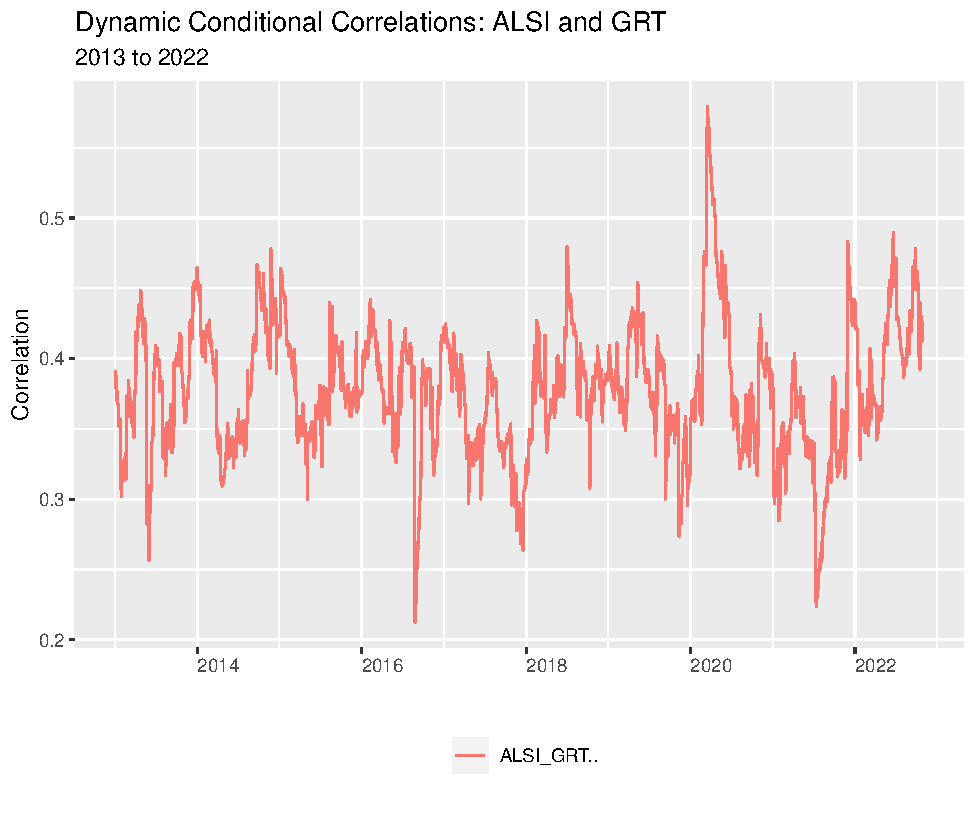
\includegraphics[width=0.5\linewidth]{Fin_Metrics_Project_files/figure-latex/figures-side-1}
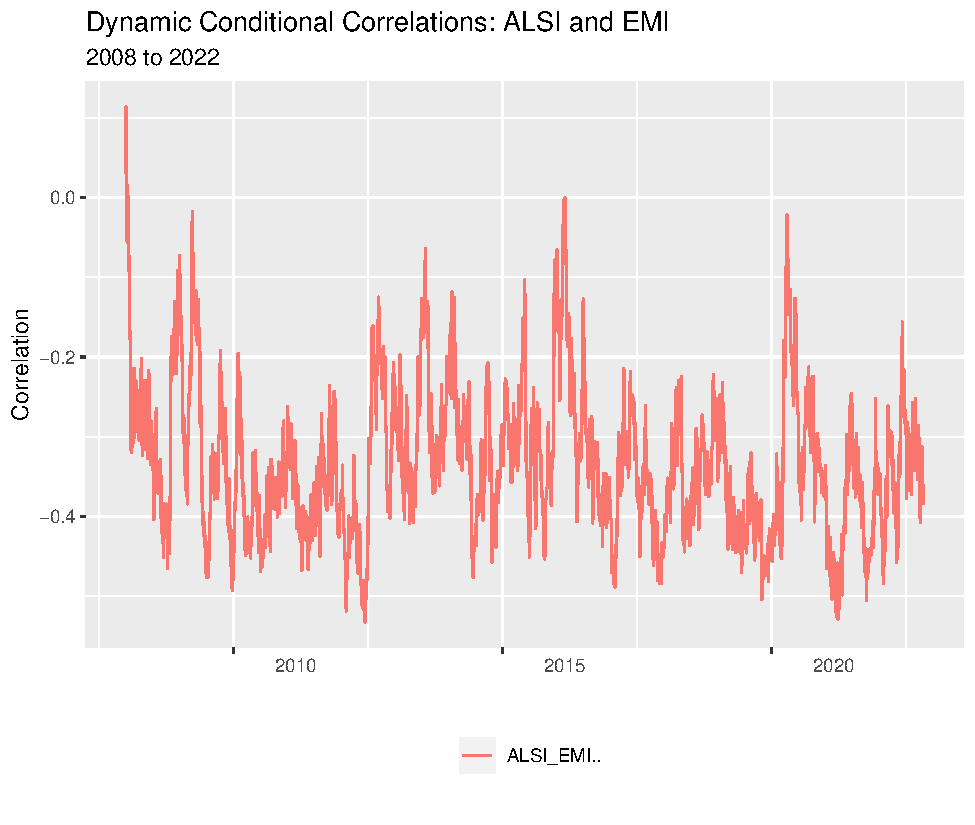
\includegraphics[width=0.5\linewidth]{Fin_Metrics_Project_files/figure-latex/figures-side-2}
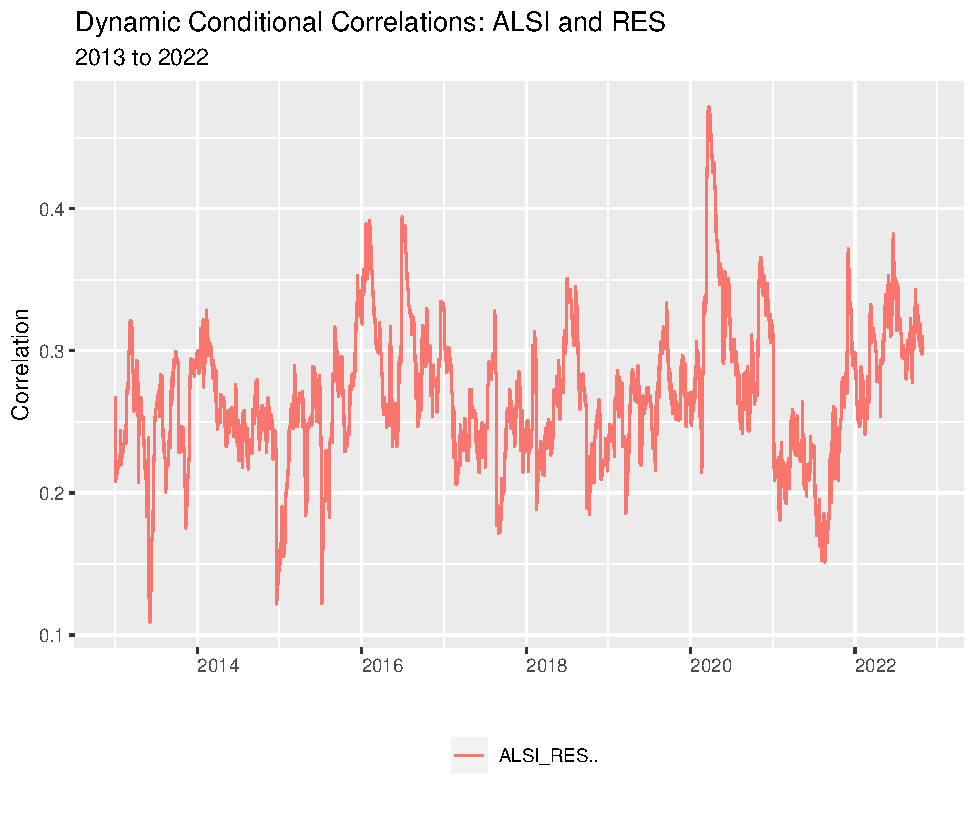
\includegraphics[width=0.5\linewidth]{Fin_Metrics_Project_files/figure-latex/figures-side-3}
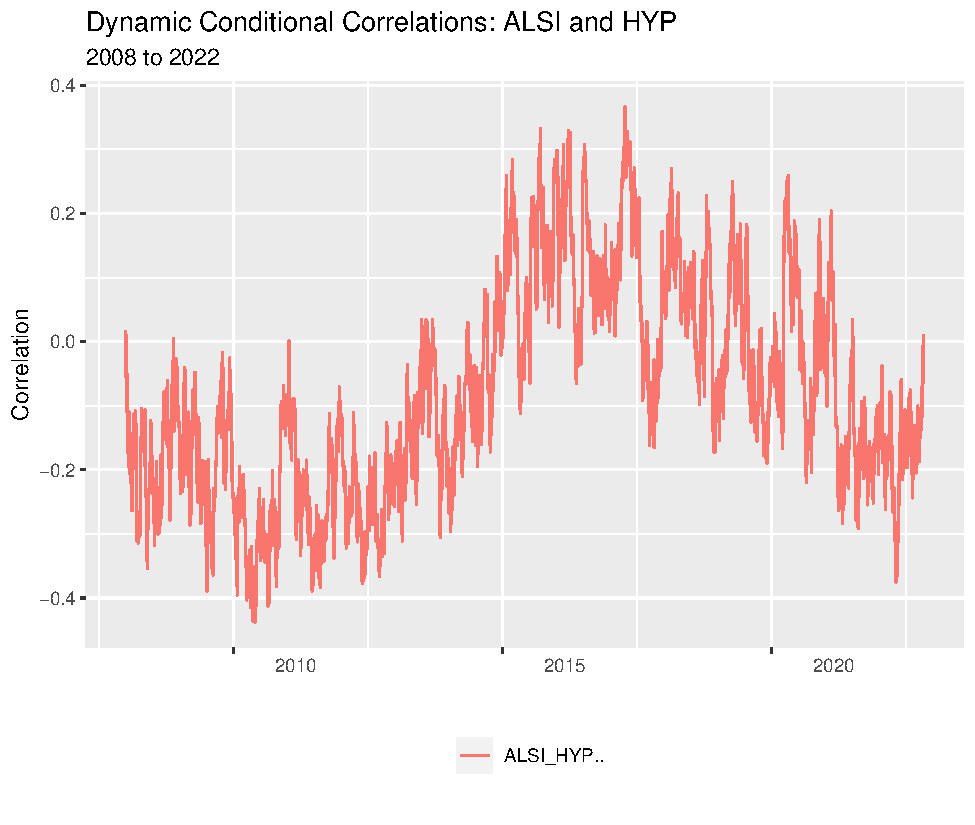
\includegraphics[width=0.5\linewidth]{Fin_Metrics_Project_files/figure-latex/figures-side-4}
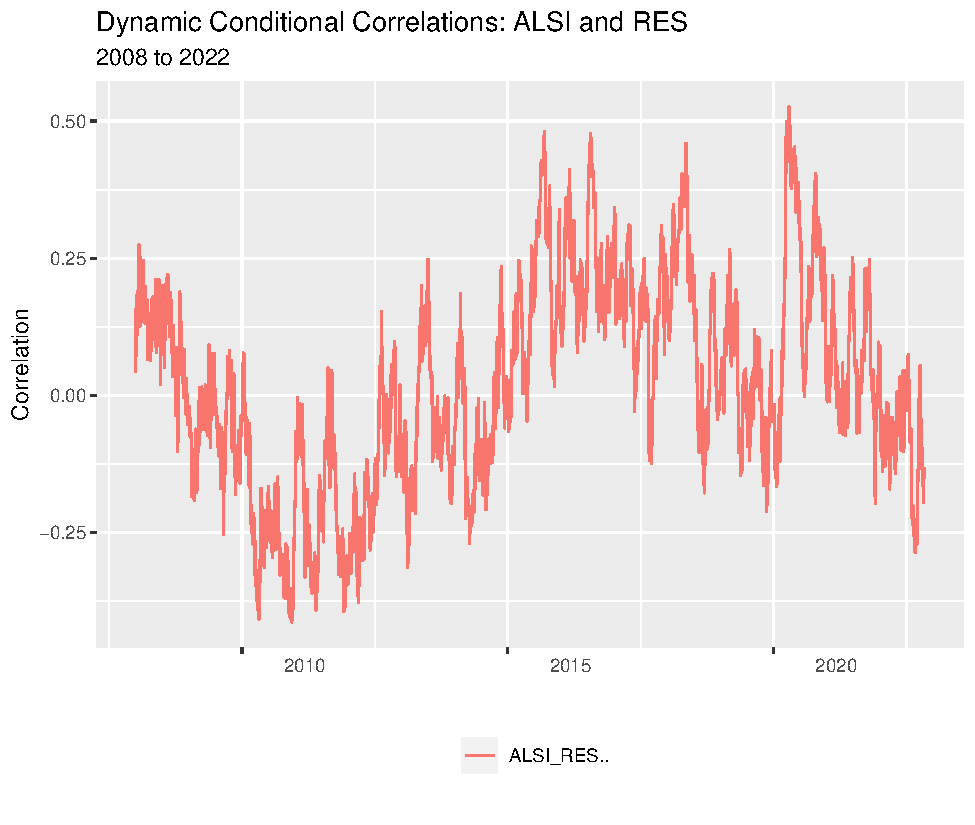
\includegraphics[width=0.5\linewidth]{Fin_Metrics_Project_files/figure-latex/figures-side-5}
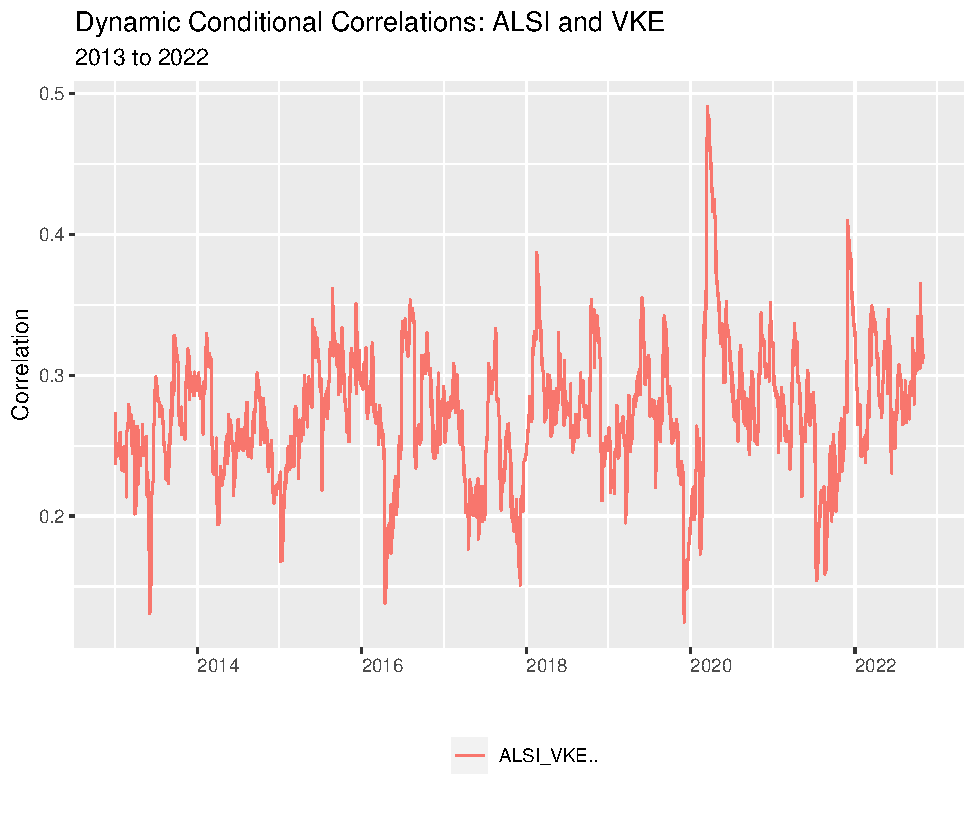
\includegraphics[width=0.5\linewidth]{Fin_Metrics_Project_files/figure-latex/figures-side-6}

\hypertarget{time-varying-correlation-periods-of-high-and-low-volatility}{%
\subsection{Time-varying Correlation: Periods of High and Low
Volatility}\label{time-varying-correlation-periods-of-high-and-low-volatility}}

In this section, periods of high USD/ZAR (Dollar Rand) volatility are
isolated and used as to filter for the ALSI combined and imputed data.
The premise being that periods of high Rand volatility can act as an
indicator for high levels of volatility in South Africa financial
markets and other asset classes. These highly volatile periods are then
used as an index to filter the returns data for periods where South
African markets were volatile.

Given that the high volatility combine imputed ALSI returns data will
have large missing gaps due to periods of moderate or low volatility,
dynamic correlations between equity pairs will have to be charted for
short periods of a time. This is due to the fact that the graphing
function used will not skip whole year periods.

Following this methodology of running multiple DCC models on smaller
periods of high volatility decreases the run time of the model.

\hypertarget{periods-of-high-and-low-volatility}{%
\subsubsection{Periods of High and Low
Volatility}\label{periods-of-high-and-low-volatility}}

When comparing the time-varying conditional correlations between the
returns of the property sector and the ALSI for periods of high and low
South African Rand volatility that there is a considerable differences
in correlation coefficients. For periods of high Rand volatility the
approximate average correlation is 0.5 whereas for period of low Rand
volatility the approximate average correlation is 0.3. Thus, in periods
of high Rand volatility macroeconomic events are having a greater effect
on REIT returns. Practically speaking the understanding of how this
relationship between the returns of the property sector and the ALSI
during periods of high and low can inform investors how the level of
diversification can change when factors that effect Rand price changes
have on their listed property holdings during periods of low and high
volatility. These results can be seen in Figures 4.4 and 4.5

\begin{figure}
\centering
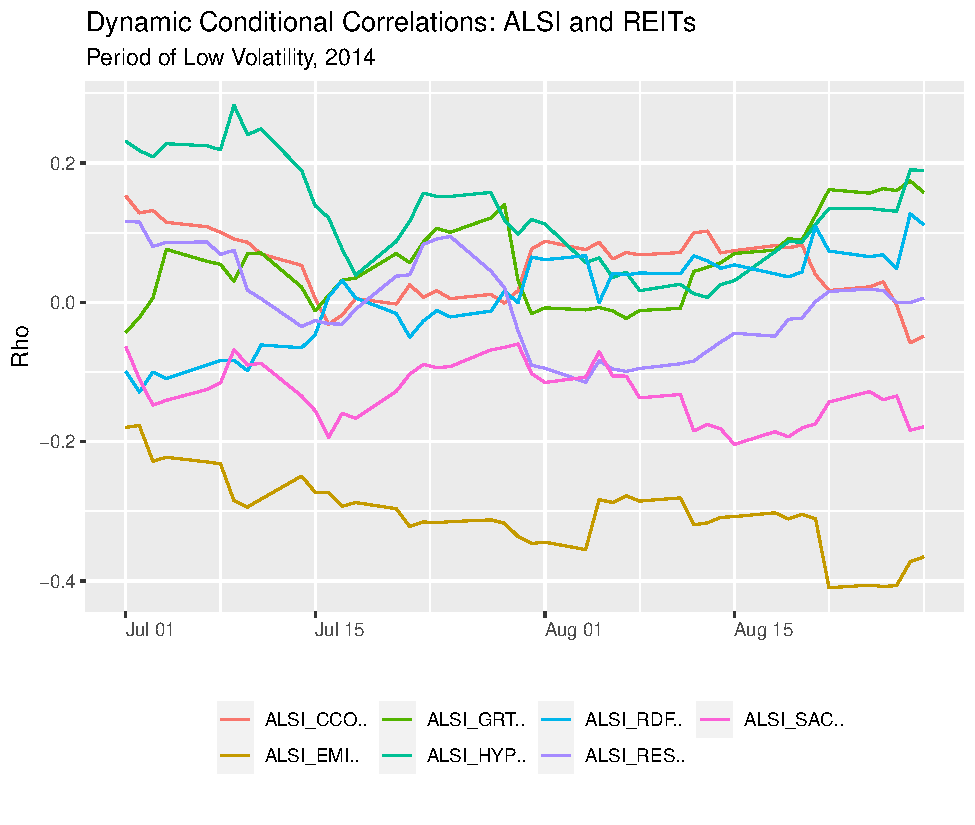
\includegraphics{Fin_Metrics_Project_files/figure-latex/unnamed-chunk-12-1.pdf}
\caption{Dynamic Conditional Correlations Graph}
\end{figure}

\begin{figure}
\centering
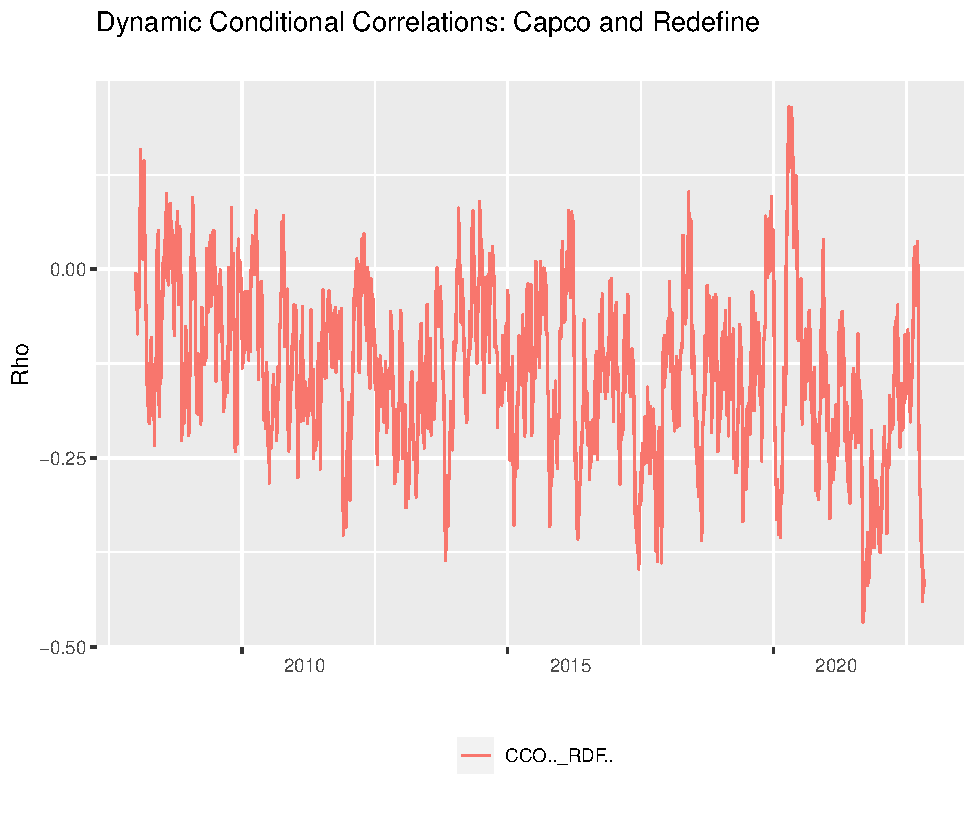
\includegraphics{Fin_Metrics_Project_files/figure-latex/unnamed-chunk-14-1.pdf}
\caption{Dynamic Conditional Correlations Graph}
\end{figure}

\hypertarget{capital-counties-properties-plc-and-redefine-properties-limited}{%
\subsection{Capital \& Counties Properties PLC and Redefine Properties
Limited}\label{capital-counties-properties-plc-and-redefine-properties-limited}}

This section applies similar techniques as discussed above between two
JSE listed REITs namely, Capital \& Counties Properties PLC and Redefine
Properties Limited. Capital \& Counties Properties PLC is a listed
company based in the United Kingdom and focuses on developments in
London whereas Redefine Properties Limited is a listed REIT with large
South African holdings.

For the period June 2018 to October 2022 the conditionally correlation
for RDF and the ALIS as well as COO and the ALSI. From Figure 4.6, prior
to 2020 there did exist a signification difference in average
approximate time-varying correlation coefficient with a coefficient of
0.25 for COO and 0.4 for RDF indicating differences in location of
assets and income structures. However, with the onset of the pandemic
followed by the high global inflation and tighter monetary policy across
the globe the correlation between returns has since narrowed, but
towards the end of 2022 the this spread has begun to increase again and
COO may offer investors a Rand hedge and further diversification to the
ALSI then RDF can offer. Figure 4.7 demonstrates how the average
correlation between the returns of COO and RDF have changed over this
four year period. It appears as the the correlation coefficient has
increased especially since the pandemic. This may confirm that during
periods of higher volatility global factors have a greater and more
similar affect on returns which can be observed in figures 4.8 and 4.9.

\begin{figure}
\centering
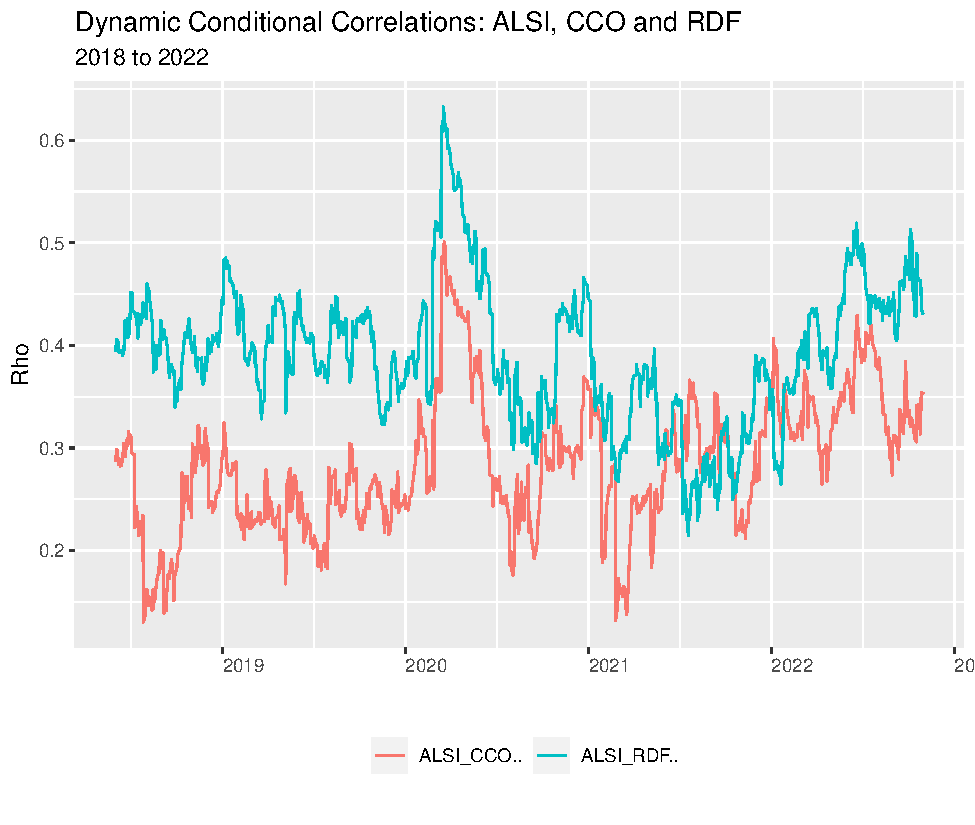
\includegraphics{Fin_Metrics_Project_files/figure-latex/unnamed-chunk-16-1.pdf}
\caption{Dynamic Conditional Correlations Graph}
\end{figure}

\begin{figure}
\centering
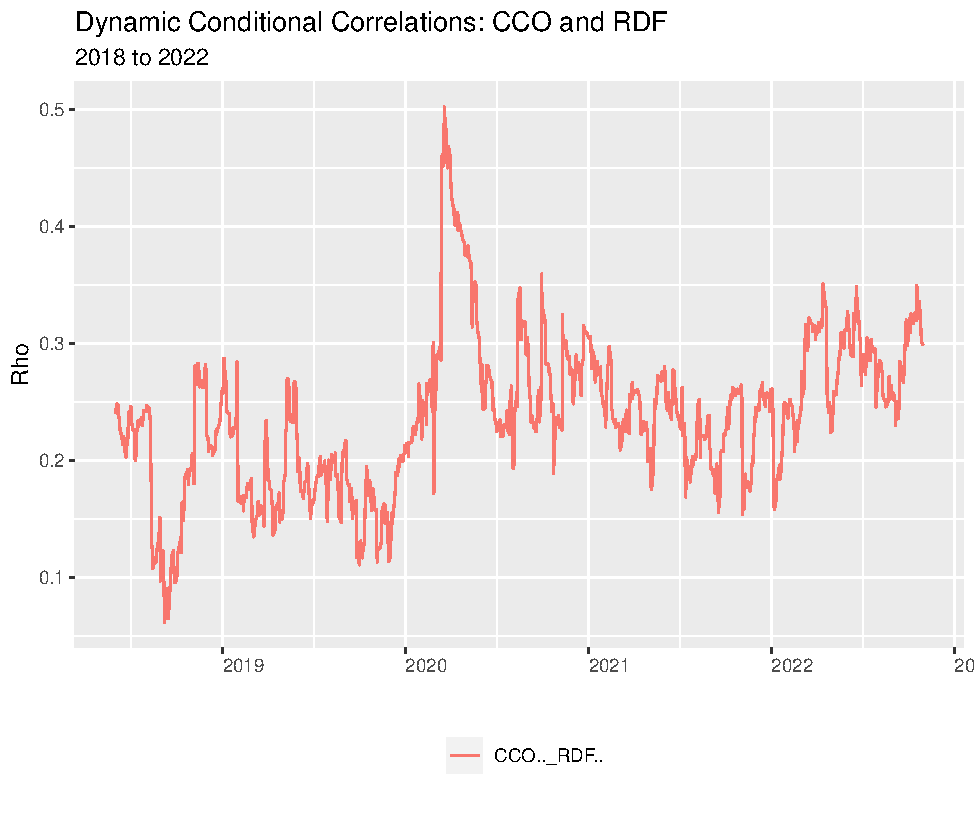
\includegraphics{Fin_Metrics_Project_files/figure-latex/unnamed-chunk-17-1.pdf}
\caption{Dynamic Conditional Correlations Graph}
\end{figure}

\begin{figure}
\centering
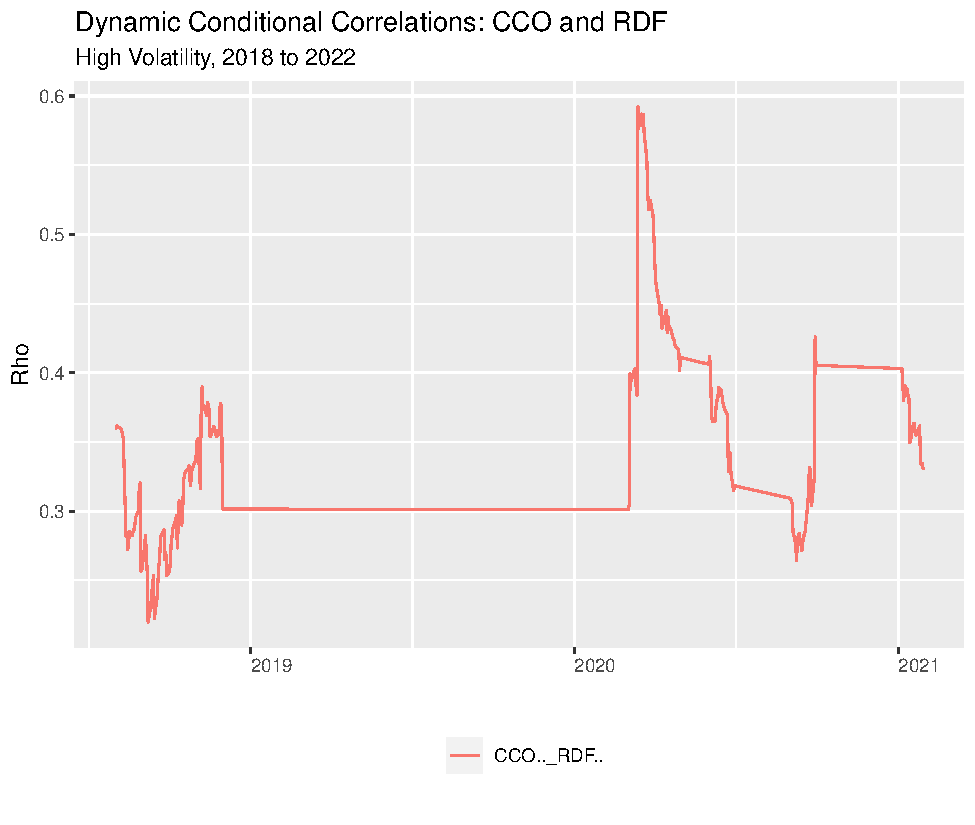
\includegraphics{Fin_Metrics_Project_files/figure-latex/unnamed-chunk-19-1.pdf}
\caption{Dynamic Conditional Correlations Graph}
\end{figure}

\begin{figure}
\centering
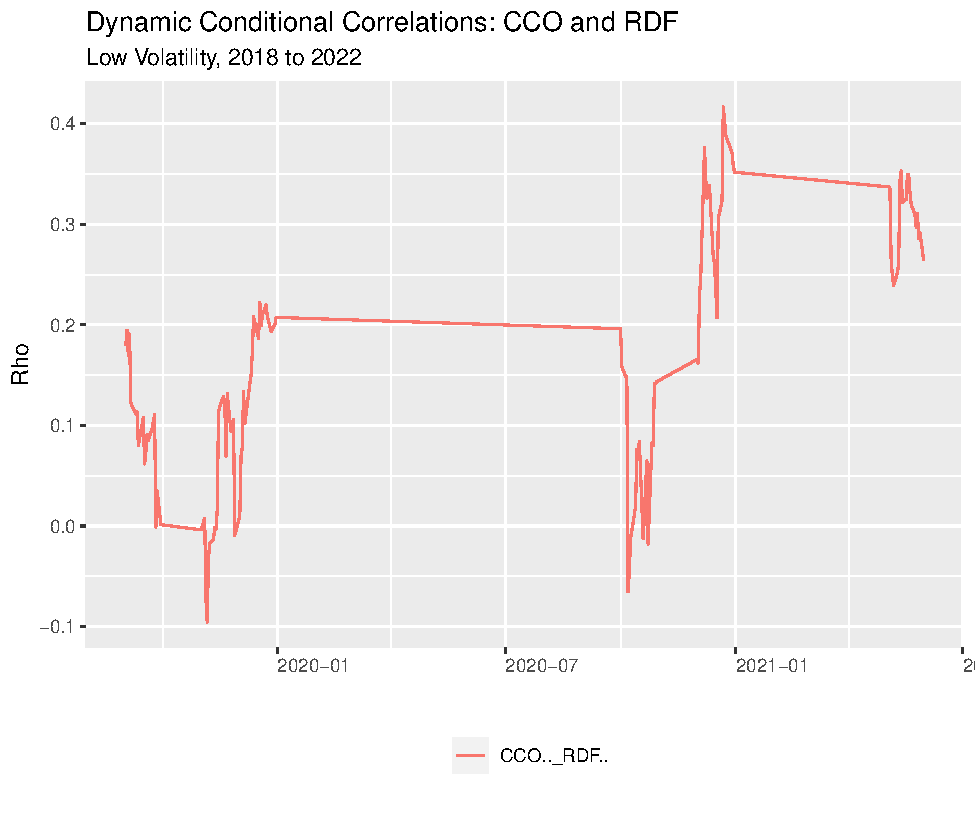
\includegraphics{Fin_Metrics_Project_files/figure-latex/unnamed-chunk-21-1.pdf}
\caption{Dynamic Conditional Correlations Graph}
\end{figure}

\hypertarget{conclusion}{%
\section{\texorpdfstring{Conclusion
\label{Conclusion}}{Conclusion }}\label{conclusion}}

One potential rationalisation for this low correlation between the
selected REITs and other JSE listed equities may be that due to the
nature of REITs, that is their diversified income stream. The
implication being that REITs receive income from tenants across various
industries, whether is be income from commercial or residential
properties only adds to the diversification of this income stream. If
one industry, other than property, experiences substantial volatility in
its return profile, again by the nature of the income stream, the impact
of any losses in rental income will be muted by other more stable
industries. Thus, the explanation for such low correlation returns
structures can be concluded as broad macro volatility experienced by
country wide factors such as currency volatility, increased money
supply, global or national level recession.

A consideration that must be made is that only when an asset is as
liquid as the other assets it is being compared to, may one be able to
ascertain whether its true correlation structure with other assets. The
research that listed equity receive and considerable transactions by
brokers and traders keep prices relatively up to date in terms of prices
reflecting new information. Thus, prior to the 2013 REIT legislation it
may be that not all relevant information was not priced into property
stocks.

Since the introduction of the REITs legislation the correlation
coefficient of returns of the SA REITs sector and the ALSI excluding
REITs appears to be increasing over the sample period. This trend may be
a result of property stocks having become mode similar to traditional
equities post legislation. This may be explained by the increased
liquidity in trading REIT shares on exchanges, making REITs more
competitive and accessible to foreign makes, increased offshore
holdings, debt ratios and greatly increased market capitalization of the
sector. That being said REITs do offer investors options to greater
diversify their portfolios and provide Rand hedges, however one must
consider prevailing macroeconomic conditions not only with the view that
it will effect one's portfolio returns, but that these conditions will
affect how truly diversified a portfolio is.

\newpage

\hypertarget{references}{%
\section*{References}\label{references}}
\addcontentsline{toc}{section}{References}

Katzler, S. and Song, H. (2017). Public real estate-correlation and
volatility dynamics in the U.K. mixed-asset portfolio. Advanced Research
in Scientific Areas, December, Pg 38-47.

Carstens, R. and Wesson, N. (2019). The impact of South African real
estate investment trust legislation on firm growth and firm value, South
African Journal of Economic and Management Sciences 22(1), Pg 2-8.

Boshoff, D. and Bredell, E. (2013). Introduction of REITs in South
Africa Transformation of the Listed Property Sector. Advanced Research
in Scientific Areas, December, Pg 2-11.

Engle, R. (2002) Dynamic Conditional Correlation: A Simple Class of
Multivariate Generalized Autoregressive Conditional Heteroskedasticity
Models. Journal of Business \& Economic Statistics, 20, 339-350.

FTSE Russel (2023). FTSE/JSE All Share Index. Available at:
\url{https://research.ftserussell.com/Analytics/Factsheets/Home}
(Accessed: 29 January 2023).

Katzke, N.F. (2022a). Practical 2 Bonus: Stratification Example.
Available at:
\url{https://www.fmx.nfkatzke.com/posts/2020-08-07-practical-2/notes/practical_2_stratifi}
(Accessed: 27 January 2023).

Katzke, N.F. (2022b). Practical 7: Multi-variate Volatility Modelling.
Available at:
\url{https://www.fmx.nfkatzke.com/posts/2020-08-17-practical-7/notes/practical_7}
(Accessed: 19 January 2023).

Katzke, N.F. (2022c). Topic 6: Multivariate Volatility Models. Available
at:
\url{https://www.fmx.nfkatzke.com/posts/2020-08-15-theory5/Notes/Session_5.pdf}
(Accessed: 30 January 2023).

National Treasury of South Africa. (2007). Reforming the listed property
sector in South Africa, response document issued by the National
Treasury. Discussion paper, Pretoria, 1-39.

Ndlovu, K. (2019). SA listed property facing challenges. STANLIB.
Available at:
\url{https://research.ftserussell.com/Analytics/Factsheets/Home}
(Accessed: 28 January 2023).

South African Reserve Bank: SARB (2023). SELECTED HISTORICAL RATES.
Available at:
\url{https://www.resbank.co.za/en/home/what-we-do/statistics/key-statistics/selected-historical-rates}
(Accessed: 28 January 2023).

\newpage

\hypertarget{annexure-a}{%
\section*{Annexure A}\label{annexure-a}}
\addcontentsline{toc}{section}{Annexure A}

\begin{figure}
\centering
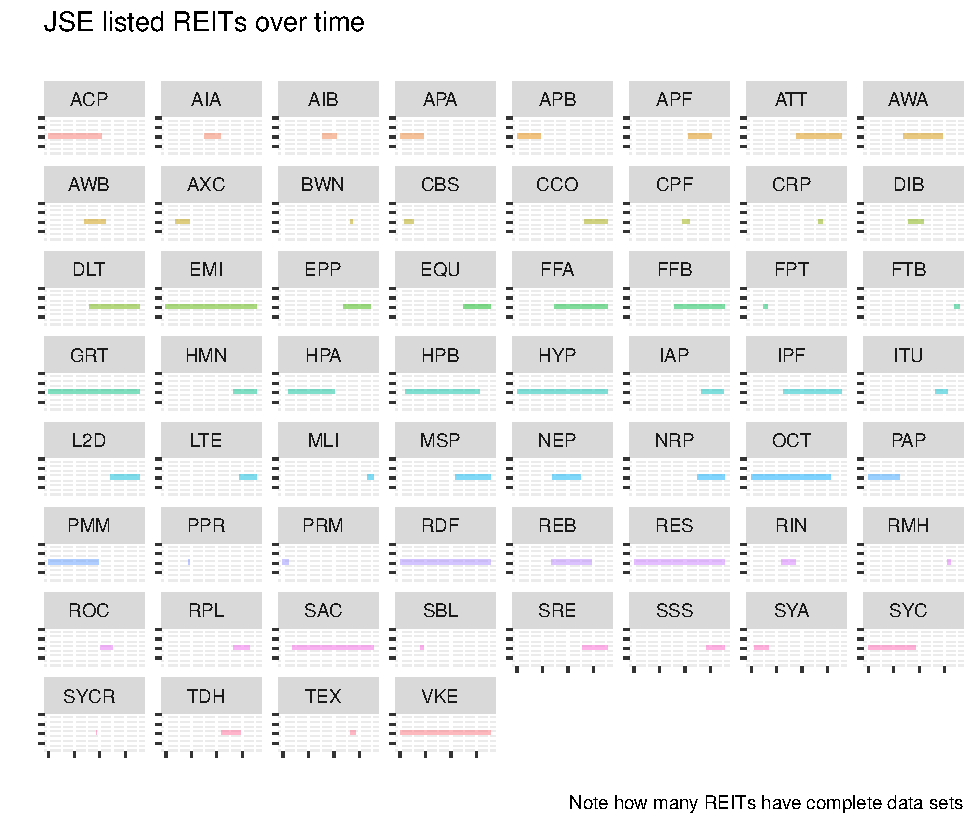
\includegraphics{Fin_Metrics_Project_files/figure-latex/unnamed-chunk-22-1.pdf}
\caption{REITs Dataset}
\end{figure}

\bibliography{Tex/ref}





\end{document}
